\documentclass[11pt]{article}


%\parindent0pt
\setlength{\headheight}{1.1\baselineskip}
\setlength{\oddsidemargin}{0cm}
\setlength{\evensidemargin}{0cm}
%\setlength{\marginparwidth}{57pt}
%\setlength{\footskip}{30pt}
\textwidth=17cm
%\hoffset=0.5cm
\textheight=24cm
\voffset=-2.5cm

%\usepackage{showkeys}


\usepackage{graphicx}
\usepackage{xcolor}
\usepackage{amsfonts,amssymb,amsmath}
\usepackage{amsthm}
\usepackage{tikz}
\usetikzlibrary{arrows, decorations.markings}
\tikzset{>=latex}

\newtheorem{definition}{Definition}
\newtheorem{theorem}{Theorem}
\newtheorem{proposition}{Proposition}
\newtheorem{lemma}{Lemma}
\newtheorem{corollary}{Corollary}
\newtheorem{remark}{Remark}
\graphicspath{{figures/}}


\def\beq{\begin{equation}}
\def\eeq{\end{equation}}

\def\H{{\mathcal H}}
\newcommand{\C}{\mathbb{C}}
\newcommand{\Z}{\mathbb{Z}}


\title{$\ell^p$-norms and optimal windows}
\author{B. Ricaud}
\date{\today}

\begin{document}
\maketitle


%%%%%%%%%%%%
\section{Introduction}
We consider the following problem:
$$\max_{g,\|g\|_2=1} \| {\cal V}_g(f)\|_p^p=\max_{g,\|g\|_2=1}  \sum_{j,k}|\langle M_kT_jg , f\rangle |^p
$$
with $p\ge 2$.
\section{Functional derivative and solution}
\subsection{At infinity}
We have the following result:
$$\lim_{p\to\infty}\left(\sum_{j,k}|\langle M_kT_jg , f\rangle |^p\right)^{1/p}=\max_{j,k}|\langle M_kT_jg , f\rangle |
$$
The maximun of the scalar product is attained when  $M_kT_jg=f$. The optimal window is equal to the signal (up to a translation and modulation).

\subsection{For $p>2$}
Introduce $A=|\langle M_kT_jg , f\rangle |^2$, its derivative with respect to $\overline{g}$ is:
$$A'(g)=\langle M_kT_jg , f\rangle T_iM_kf.
$$
One can write
$$\frac{\partial}{\partial \overline{g}}\sum_{j,k}|\langle M_kT_jg , f\rangle |^p=\sum_{j,k}\frac{\partial}{\partial \overline{g}}A^{p/2}(g)=\frac{p}{2}\sum_{j,k} A(g)^{\frac{p}{2}-1} A'(g)
$$
The optimal $g$ is given by the solution of
$$\frac{p}{2}\sum_{j,k}  |\langle M_kT_jg , f\rangle |^{\frac{p}{2}-1}  \langle M_kT_jg , f\rangle T_iM_kf=\lambda g
$$
with $\lambda$ the smallest eigenvalue of the Gabor multiplier with mask $A(g)^{\frac{p}{2}-1} $.
{\color{red} For $p$ close to 2, for our signals the optimal windows look like chirped Gaussians. Is there a simple way to explain that? It is not always true since for example we managed to obtain a square-shaped window for $f$ being a square in the TF plane in our EUSIPCO paper (by solving the above eigenvalue problem).}


\subsection{Near two}
Introduce $\gamma=2-p$. One can write
\begin{align}
A^\gamma=\exp(p\ln A)=1+\gamma\ln A+\gamma^2\ln^2 A+\cdots
\end{align}
For $p$ tends to two the $L^p$-norm becomes:
\begin{align*}
\sum_{j,k}|\langle M_kT_jg , f\rangle |^p&=\sum_{j,k}|\langle M_kT_jg , f\rangle |^2 |\langle M_kT_jg , f\rangle |^\gamma\\
&=1+\frac{\gamma}{2} \sum_{j,k}|\langle M_kT_jg , f\rangle |^2 \ln|\langle M_kT_jg , f\rangle |^2+{\cal O}(\gamma^2)
\end{align*}
The derivative with respect to $\overline{g}$ gives: 
$$A'(g)=\langle M_kT_jg , f\rangle T_iM_kf,
$$
and
$$(A\ln A)'=A'(1+\ln A).
$$
Notice that if $\{T_iM_kf\}$ is a tight frame,
$$\sum A'=g.
$$
So that the extremum of the $\ell^p$-norm is the solution of (case of tight frame):
$$-\sum_{j,k}\ln|\langle M_kT_jg , f\rangle |^2\langle g , T_jM_kf\rangle T_iM_kf=g+\lambda g.
$$
One has to diagonalize the gabor multiplier with mask
$$M=-\ln|\langle M_kT_jg , f\rangle |^2.
$$

%%%%%%%%%%%%%%%%%%%%%%%%%%%
\section{Optimization in the subclass of chirped Gaussians}

Since the optimization problem with a small value for $p$ leads to a chirped Gaussian-like atom, it may be more convenient to directly search for a solution in the subclass of chirped Gaussians. Let us introduce the subclass $\cal G$ of chirped Gaussian in $\C^N$. A function in this space is of the form $M_kT_j\phi_{\sigma,s}$ where
\begin{equation}\label{Gaussianeq}
\phi_{\sigma,s}(t)=\sqrt[4]{\frac{2}{N\sigma}}e^{-\pi\frac{t^2}{N\sigma}+i \pi s \frac{t^2}{N}},
\end{equation}
where $\sigma$ is positive and $s$ is a real number.

We want to maximize the following quantity over $\sigma$ and $s$:
$$\|{\cal V}_{\phi_{\sigma,s}}f\|^p,
$$
where $p>2$.
\subsection{Gradient step}
The gradient is given by
\begin{align}
\frac{\partial \|{\cal V}_{\phi_{\sigma,s}}f\|^p}{\partial \sigma}=p\ \text{Re}[\langle G_{f,M}\phi_{\sigma,s},\frac{\partial \phi_{\sigma,s}}{\partial \sigma}\rangle],\\
\frac{\partial \|{\cal V}_{\phi_{\sigma,s}}f\|^p}{\partial s}=p\ \text{Re}[\langle G_{f,M}\phi_{\sigma,s},\frac{\partial \phi_{\sigma,s}}{\partial s}\rangle],
\end{align}
where $G_{f,M}$ is the Gabor multiplier with window $f$ and mask $M=|\langle M_kT_jf , \phi_{\sigma,s}\rangle |^{p-2}$. One can see it by writing for $p>2$ even, any window $g$ and function $f$:
\begin{align*}
\sum_{j,k}|\langle M_kT_jg , f\rangle |^p&=\sum_{j,k}\langle M_kT_jg , f\rangle^{p/2} \langle f,M_kT_jg \rangle^{p/2}
\end{align*}
and 
$$\frac{\partial}{\partial s}\langle M_kT_j\phi_{\sigma,s} , f\rangle^{p/2}=\frac{p}{2}\langle \frac{\partial}{\partial s}\phi_{\sigma,s} , T_jM_kf\rangle \langle \phi_{\sigma,s} , T_jM_kf\rangle^{p/2-1}.
$$
At each step of the gradient method, one compute:
\begin{align}
\sigma_{n+1}&=\sigma_n+\alpha p\ \text{Re}[\langle G_{f,M^{(n)}}\phi_{\sigma,s}^{(n)},\frac{\partial \phi_{\sigma,s}^{(n)}}{\partial \sigma}\rangle]\\
s_{n+1}&=s_n+\alpha p\ \text{Re}[\langle G_{f,M^{(n)}}\phi_{\sigma,s}^{(n)},\frac{\partial \phi_{\sigma,s}^{(n)}}{\partial s}\rangle]
\end{align}
and $\phi_{\sigma,s}^{(n+1)}=\phi_{\sigma_{n+1},s_{n+1}}$.

The derivatives of the function $\phi_{\sigma,s}$ with respect to $\sigma$ and $s$ read:
$$\frac{\partial \phi_{\sigma,s}}{\partial \sigma}(t)= \left(\frac{\pi t^2}{\sigma^2 N}-\frac{1}{4\sigma}\right)\phi_{\sigma,s}(t)
$$
and
$$\frac{\partial \phi_{\sigma,s}}{\partial s}(t)=  \frac{i\pi}{N} t^2 \phi_{\sigma,s}(t).
$$

%%%%%%%%%%%%%%%%
\subsection{Hessian and Newton's method}
In order to calculate the Hessian matrix we would need the second derivatives with respect to the parameters:
\begin{align}
\frac{\partial^2}{\partial s^2}\phi_{\sigma,s}(t)&=-\left(\frac{\pi t^2}{N}\right)^2\phi_{\sigma,s}(t)\\
\frac{\partial^2}{\partial s\partial\sigma}\phi_{\sigma,s}(t)&=i\frac{\pi t^2}{N}\left(\frac{\pi t^2}{\sigma^2 N}-\frac{1}{4\sigma}\right)\phi_{\sigma,s}(t)\\
\frac{\partial^2}{\partial \sigma^2}\phi_{\sigma,s}(t)&=\left[\frac{1}{4\sigma^2}-\frac{2\pi t^2}{N\sigma^3}+\left(\frac{\pi t^2}{\sigma^2 N}-\frac{1}{4\sigma}\right)^2\right]\phi_{\sigma,s}(t)
\end{align}
{\color{red} However, the derivative of the whole cost function leads to an operation which is not a Gabor multiplier...}

%%%%%%%%%%%%%%%%%%%%%%%
\subsection{Lattice parameters}

In this section we present a way to provide the most appropriate lattice to our optimal window. For example if the window is a round shaped Gaussian, the best lattice is the quincux lattice as it packs the atoms in an optimal manner.
 
Our optimal windows are ellipsis-shaped atoms in the TF plane. They are characterized in the TF plane by their  excentricity $e=L/l$ where $l$ and $L$ are the small and large diameter respectively. In addition, the ellipsis has an orientation given by the direction parallel to the large diameter. The difference from the horizontal direction is given by a shear parameter $s$.
\begin{figure}
\center
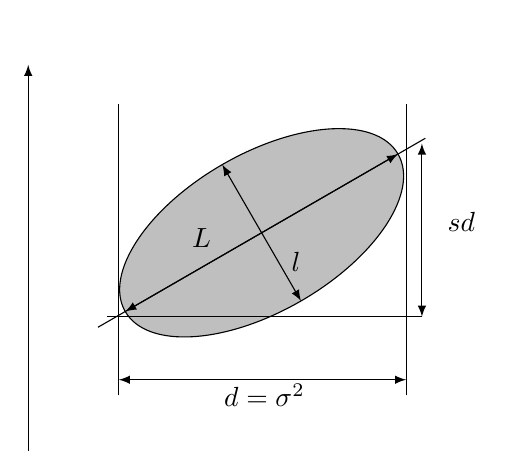
\begin{tikzpicture}
%    \shorthandoff{:;!?};
 %   \draw (0,-2) arc (-90:-270:1);
    \draw[->] (0,0) -- (5,0);
    \draw[->] (0,0) -- (0,5);
    \filldraw[fill=lightgray,rotate=30] (4,1) ellipse (2 and 1);
    \draw[<->] (1.15,1)--(4.8,1);
    \node at (3,0.8) {$d=\sigma^2$};
    \draw[<->,rotate=30,xshift=4cm,yshift=0cm] (0,0)--(0,2);
    \node at (3.4,2.5) {$l$};
    \draw[rotate=120,xshift=1cm,yshift=-6cm] (0,-0.4)--(0,4.4); 
    \draw[<->,rotate=120,xshift=1cm,yshift=-6cm] (0,0)--(0,4);
    \node at (2.2,2.8) {$L$};
    \draw (1.15,0.8) -- (1.15,4.5);
    \draw (4.8,0.8) -- (4.8,4.5);
    \draw (1,1.8)--(5,1.8);
    \draw[<->] (5,1.8) -- (5,4);
  \node at (5.5,3) {$sd$};
\end{tikzpicture}
\caption{Atoms parameters.}
\end{figure}
We recall the expression given in \eqref{Gaussianeq} of the optimal function:
\begin{equation}
\phi_{\sigma,s}(t)=\sqrt[4]{\frac{2}{N\sigma}}e^{-\pi\frac{t^2}{N\sigma}+i \pi s \frac{t^2}{N}}.
\end{equation}
This function is normalized such that $\|\phi_{\sigma,s}\|_2=1$. It has been chosen such that it is compatible with the LTFAT functions "pgauss" and "pchirp".
The spreading $d$ of the function along the time direction is given by $d=\sigma^2$ (variance of the Gaussian). $\sigma$ has the same effect as the parameter "tfr" of "pgauss". The shear of   the ellipsis is given by $s$ as in the function "pchirp". A chirp with slope $s$ revolves $s$ times around the time-frequency plane in frequency. Here $s$ may not be an integer. To link the excentricity and the variance, we know that a Gaussian with a variance $d$ in time has a variance $1/d$ in frequency. We can deduce the relation with the excentricity of the ellipsis:
\begin{equation}
e=\sigma^2(1+s^2).
\end{equation}



%%%%%%%%%%%%%%%%%%%%%%%
\subsection{Spread limitation}
 {\color{red} Must be revised, we can control the spreading by controlling the value of $d$. We don't really need to multiply by a weight function}

Some optimal window are too much spread in time and prevent a precise localization of the TF component in time. We introduced an additional constraint in the optimization procedure in order to control this spreading. We introduce a weight function $w$ of the form
$$w(t)=e^{-t^2/a^2}, \qquad a>0.
$$
The parameter $a$ fixes the time spreading of the optimal window.
In the gradient ascent loop, the computation is  modified at each step by adding:
$$\psi_{\sigma,s}^{(n)}=w \phi_{\sigma,s}^{(n)}.
$$
So that:
$$s_{n+1}=s_n+\nabla s,
$$
where
$$\nabla s=p\ \langle G_{f,M^{(n)}}\psi_{\sigma,s}^{(n)},\frac{\partial \psi_{\sigma,s}^{(n)}}{\partial s}\rangle,
$$
with 
$$M^{(n)}=|\langle M_kT_jf ,\psi_{\sigma,s}^{(n)}\rangle |^{p-2}.
$$
It is a sort of projection but instead of setting some coefficients to zero, we weight them with $w$. {\color{red} It is not a projection since $w\phi\neq w(w\phi)$}.




%\section{Non regular lattice}
%{\color{red} Just some things we understood.}
%Suppose the signal is a piece of circle in the TF plane. If the following lattice is chosen the TF concentration will be greatly improved: the lattice points are on concentric circles with center: the point being the center of the circle on which the TF component lies. A lattice which is only a sheared version of the regular one won't help much in that case. Sheared lattices are good only for linear chirps. Question: Does it improve \emph{a lot} the concentration if we use a sheared lattice with our linear chirp component? Does it worth it? 

 
\end{document}